% =====================================================================
% Appendix generated by gen_appendix.py (do not edit the lists by hand).
% Packages needed in the preamble: tikz, longtable, booktabs, array, xcolor, amssymb, hyperref.
% Paste after \appendix (the \tikzset and \newcommand lines may also go in the preamble).
% The \ref and \cite labels are those of the LaTeX source of the paper.
% Output of: python3 gen_appendix.py > appendix_classes.tex
% =====================================================================
\tikzset{
  poset/.style={x=0.5cm, y=0.5cm},
  pt/.style={circle, fill, inner sep=0pt, minimum size=3pt},
  cov/.style={line width=0.5pt},     % arrows instead of segments: cov/.style={-{Stealth[length=3pt]}, shorten >=1pt}
  tag/.style={below=2pt, font=\scriptsize, inner sep=1pt},
}
\newcommand{\classhead}[5]{\par\medskip\noindent\textbf{Class #1.}\ #2~poset\ifnum#2>1 s\fi,
  $\chi_P(t) = #3$\if\relax\detokenize{#4}\relax\else, type #4\fi
  \if\relax\detokenize{#5}\relax\else; #5\fi.\par\nopagebreak}
\newenvironment{posetrow}{\par\noindent\raggedright\setlength{\lineskip}{7pt}}{\par\smallskip}
\newcommand{\posetsep}{\hspace{1.4em plus 0.8em}}

\section{The \texorpdfstring{$\sim_L$}{~L}-classes of connected posets with at most six elements}
\label{app:classes}

In this appendix we list the $\sim_L$-classes of connected posets with at most six elements, up to
isomorphism. Each $\sim_L$-class is contained in a class of universal derived equivalence
(Corollary~\ref{The associated universally derived equivalent poset}). By
Theorem~\ref{thm:classification-small-posets}, for posets with at most five elements the two
coincide, and they also coincide with the classes of derived equivalence of incidence algebras over
any field; for six elements the same holds except possibly for the classes $\alpha$ and $\beta$ of
Section~\ref{the case of six elements}. For more elements, distinct $\sim_L$-classes might still
consist of universally derived equivalent posets (Section~\ref{sec:completeness}); for this reason we
speak of $\sim_L$-classes.

It suffices to consider connected posets. If $P = X \sqcup Y$ is a disjoint union, the admissible
cuts of $P$ are exactly the partitions whose restrictions to $X$ and to $Y$ are admissible cuts,
possibly with an empty part, and the associated negative poset is the disjoint union of the two
negative posets. Hence the $\sim_L$-class of a poset is determined by the $\sim_L$-classes of its
connected components.

In the diagrams, larger elements are drawn higher and each segment is a covering relation. For each
class we give the number of its posets up to isomorphism, the Coxeter polynomial $\chi_P(t)$ of
Section~\ref{Derived invariants and the census}, which is the same for all posets of the class, and
the type of the class when it contains the orientations of a tree
(Corollary~\ref{cor:trees}) or an orientation of a cycle with no two distinct directed paths with the
same endpoints. For trees we use the names $\mathbb{A}_n$, $\mathbb{D}_n$, $\mathbb{E}_6$ of Dynkin
diagrams and $\widetilde{\mathbb{D}}_n$ of Euclidean diagrams, and we write \emph{wild} for the other
trees; $\widetilde{\mathbb{A}}_{p,q}$ denotes a cycle with $p$ arrows in one direction and $q$ in the
other. When a class contains neither, no type is given; in Table~\ref{tab:app-six} this is indicated
by a dash. In particular, the label \emph{wild} is used only for classes of orientations of trees,
and a dash gives no information on the representation type of the posets in the class. Posets that appear in the text are marked below their diagrams. The diagrams and the table
were generated by the script \texttt{gen\_appendix.py} of the repository, which recomputes the classes
directly from Definition~\ref{def admissible cuts} and
Corollary~\ref{The associated universally derived equivalent poset}; the numbers of posets and of
classes agree with Table~\ref{tab:small-poset-census}.

\subsection{Connected posets with at most five elements}
\label{app:small}
For $n\le 2$ there is a single connected poset with $n$ elements. For $n=3,4,5$ we draw all $3+10+44=57$ connected posets, grouped into their $1+3+6$ classes.

\classhead{3.1}{3}{t^{3} + t^{2} + t + 1}{$\mathbb{A}_{3}$}{}
\begin{posetrow}

\begin{tikzpicture}[poset,baseline=0pt]
\node[pt] (v0) at (-0.5,0) {};
\node[pt] (v1) at (0.5,0) {};
\node[pt] (v2) at (0,1) {};
\draw[cov] (v0) -- (v2);
\draw[cov] (v1) -- (v2);
\end{tikzpicture}
\posetsep

\begin{tikzpicture}[poset,baseline=0pt]
\node[pt] (v0) at (0,0) {};
\node[pt] (v1) at (-0.5,1) {};
\node[pt] (v2) at (0.5,1) {};
\draw[cov] (v0) -- (v1);
\draw[cov] (v0) -- (v2);
\end{tikzpicture}
\posetsep

\begin{tikzpicture}[poset,baseline=0pt]
\node[pt] (v0) at (0,0) {};
\node[pt] (v1) at (0,1) {};
\node[pt] (v2) at (0,2) {};
\draw[cov] (v0) -- (v1);
\draw[cov] (v1) -- (v2);
\end{tikzpicture}
\end{posetrow}

\classhead{4.1}{4}{t^{4} + t^{3} + t^{2} + t + 1}{$\mathbb{A}_{4}$}{}
\begin{posetrow}
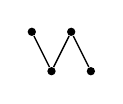
\begin{tikzpicture}[poset,baseline=0pt]
\node[pt] (v0) at (-0.5,0) {};
\node[pt] (v1) at (0.5,0) {};
\node[pt] (v2) at (-1,1) {};
\node[pt] (v3) at (0,1) {};
\draw[cov] (v0) -- (v2);
\draw[cov] (v0) -- (v3);
\draw[cov] (v1) -- (v3);
\end{tikzpicture}
\posetsep
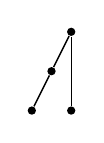
\begin{tikzpicture}[poset,baseline=0pt]
\node[pt] (v0) at (-0.5,0) {};
\node[pt] (v1) at (0.5,0) {};
\node[pt] (v2) at (0,1) {};
\node[pt] (v3) at (0.5,2) {};
\draw[cov] (v0) -- (v2);
\draw[cov] (v1) -- (v3);
\draw[cov] (v2) -- (v3);
\end{tikzpicture}
\posetsep
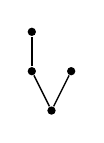
\begin{tikzpicture}[poset,baseline=0pt]
\node[pt] (v0) at (0,0) {};
\node[pt] (v1) at (-0.5,1) {};
\node[pt] (v2) at (0.5,1) {};
\node[pt] (v3) at (-0.5,2) {};
\draw[cov] (v0) -- (v1);
\draw[cov] (v0) -- (v2);
\draw[cov] (v1) -- (v3);
\end{tikzpicture}
\posetsep

\begin{tikzpicture}[poset,baseline=0pt]
\node[pt] (v0) at (0,0) {};
\node[pt] (v1) at (0,1) {};
\node[pt] (v2) at (0,2) {};
\node[pt] (v3) at (0,3) {};
\draw[cov] (v0) -- (v1);
\draw[cov] (v1) -- (v2);
\draw[cov] (v2) -- (v3);
\end{tikzpicture}
\end{posetrow}

\classhead{4.2}{5}{t^{4} + t^{3} + t + 1}{$\mathbb{D}_{4}$}{$I_2\times I_2$, Example~\ref{ex:D4-square}}
\begin{posetrow}
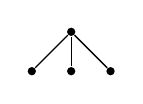
\begin{tikzpicture}[poset,baseline=0pt]
\node[pt] (v0) at (-1,0) {};
\node[pt] (v1) at (0,0) {};
\node[pt] (v2) at (1,0) {};
\node[pt] (v3) at (0,1) {};
\draw[cov] (v0) -- (v3);
\draw[cov] (v1) -- (v3);
\draw[cov] (v2) -- (v3);
\end{tikzpicture}
\posetsep
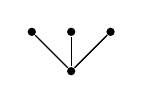
\begin{tikzpicture}[poset,baseline=0pt]
\node[pt] (v0) at (0,0) {};
\node[pt] (v1) at (-1,1) {};
\node[pt] (v2) at (0,1) {};
\node[pt] (v3) at (1,1) {};
\draw[cov] (v0) -- (v1);
\draw[cov] (v0) -- (v2);
\draw[cov] (v0) -- (v3);
\end{tikzpicture}
\posetsep
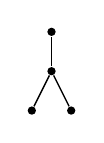
\begin{tikzpicture}[poset,baseline=0pt]
\node[pt] (v0) at (-0.5,0) {};
\node[pt] (v1) at (0.5,0) {};
\node[pt] (v2) at (0,1) {};
\node[pt] (v3) at (0,2) {};
\draw[cov] (v0) -- (v2);
\draw[cov] (v1) -- (v2);
\draw[cov] (v2) -- (v3);
\end{tikzpicture}
\posetsep
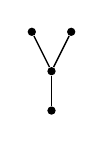
\begin{tikzpicture}[poset,baseline=0pt]
\node[pt] (v0) at (0,0) {};
\node[pt] (v1) at (0,1) {};
\node[pt] (v2) at (-0.5,2) {};
\node[pt] (v3) at (0.5,2) {};
\draw[cov] (v0) -- (v1);
\draw[cov] (v1) -- (v2);
\draw[cov] (v1) -- (v3);
\end{tikzpicture}
\posetsep
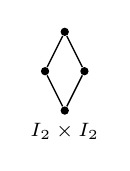
\begin{tikzpicture}[poset,baseline=0pt]
\node[pt] (v0) at (0,0) {};
\node[pt] (v1) at (-0.5,1) {};
\node[pt] (v2) at (0.5,1) {};
\node[pt] (v3) at (0,2) {};
\draw[cov] (v0) -- (v1);
\draw[cov] (v0) -- (v2);
\draw[cov] (v1) -- (v3);
\draw[cov] (v2) -- (v3);
\node[tag] at (current bounding box.south) {$I_2\times I_2$};
\end{tikzpicture}
\end{posetrow}

\classhead{4.3}{1}{t^{4} - 2t^{2} + 1}{$\widetilde{\mathbb{A}}_{2,2}$}{$2\oplus2$, Proposition~\ref{prop:ordinal-sums}}
\begin{posetrow}
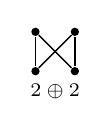
\begin{tikzpicture}[poset,baseline=0pt]
\node[pt] (v0) at (-0.5,0) {};
\node[pt] (v1) at (0.5,0) {};
\node[pt] (v2) at (-0.5,1) {};
\node[pt] (v3) at (0.5,1) {};
\draw[cov] (v0) -- (v2);
\draw[cov] (v0) -- (v3);
\draw[cov] (v1) -- (v2);
\draw[cov] (v1) -- (v3);
\node[tag] at (current bounding box.south) {$2\oplus2$};
\end{tikzpicture}
\end{posetrow}

\classhead{5.1}{10}{t^{5} + t^{4} + t^{3} + t^{2} + t + 1}{$\mathbb{A}_{5}$}{}
\begin{posetrow}
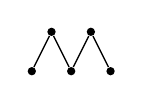
\begin{tikzpicture}[poset,baseline=0pt]
\node[pt] (v0) at (0,0) {};
\node[pt] (v1) at (-1,0) {};
\node[pt] (v2) at (1,0) {};
\node[pt] (v3) at (-0.5,1) {};
\node[pt] (v4) at (0.5,1) {};
\draw[cov] (v0) -- (v3);
\draw[cov] (v0) -- (v4);
\draw[cov] (v1) -- (v3);
\draw[cov] (v2) -- (v4);
\end{tikzpicture}
\posetsep
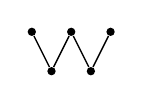
\begin{tikzpicture}[poset,baseline=0pt]
\node[pt] (v0) at (-0.5,0) {};
\node[pt] (v1) at (0.5,0) {};
\node[pt] (v2) at (-1,1) {};
\node[pt] (v3) at (1,1) {};
\node[pt] (v4) at (0,1) {};
\draw[cov] (v0) -- (v2);
\draw[cov] (v0) -- (v4);
\draw[cov] (v1) -- (v3);
\draw[cov] (v1) -- (v4);
\end{tikzpicture}
\posetsep
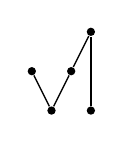
\begin{tikzpicture}[poset,baseline=0pt]
\node[pt] (v0) at (-0.5,0) {};
\node[pt] (v1) at (0.5,0) {};
\node[pt] (v2) at (0,1) {};
\node[pt] (v3) at (-1,1) {};
\node[pt] (v4) at (0.5,2) {};
\draw[cov] (v0) -- (v2);
\draw[cov] (v0) -- (v3);
\draw[cov] (v1) -- (v4);
\draw[cov] (v2) -- (v4);
\end{tikzpicture}
\posetsep
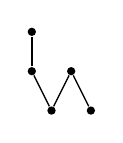
\begin{tikzpicture}[poset,baseline=0pt]
\node[pt] (v0) at (-0.5,0) {};
\node[pt] (v1) at (0.5,0) {};
\node[pt] (v2) at (-1,1) {};
\node[pt] (v3) at (0,1) {};
\node[pt] (v4) at (-1,2) {};
\draw[cov] (v0) -- (v2);
\draw[cov] (v0) -- (v3);
\draw[cov] (v1) -- (v3);
\draw[cov] (v2) -- (v4);
\end{tikzpicture}
\posetsep
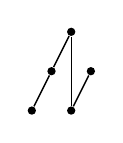
\begin{tikzpicture}[poset,baseline=0pt]
\node[pt] (v0) at (-0.5,0) {};
\node[pt] (v1) at (0.5,0) {};
\node[pt] (v2) at (0,1) {};
\node[pt] (v3) at (1,1) {};
\node[pt] (v4) at (0.5,2) {};
\draw[cov] (v0) -- (v2);
\draw[cov] (v1) -- (v3);
\draw[cov] (v1) -- (v4);
\draw[cov] (v2) -- (v4);
\end{tikzpicture}
\posetsep
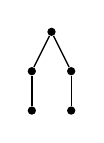
\begin{tikzpicture}[poset,baseline=0pt]
\node[pt] (v0) at (-0.5,0) {};
\node[pt] (v1) at (0.5,0) {};
\node[pt] (v2) at (-0.5,1) {};
\node[pt] (v3) at (0.5,1) {};
\node[pt] (v4) at (0,2) {};
\draw[cov] (v0) -- (v2);
\draw[cov] (v1) -- (v3);
\draw[cov] (v2) -- (v4);
\draw[cov] (v3) -- (v4);
\end{tikzpicture}
\posetsep
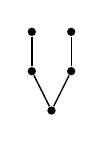
\begin{tikzpicture}[poset,baseline=0pt]
\node[pt] (v0) at (0,0) {};
\node[pt] (v1) at (-0.5,1) {};
\node[pt] (v2) at (0.5,1) {};
\node[pt] (v3) at (-0.5,2) {};
\node[pt] (v4) at (0.5,2) {};
\draw[cov] (v0) -- (v1);
\draw[cov] (v0) -- (v2);
\draw[cov] (v1) -- (v3);
\draw[cov] (v2) -- (v4);
\end{tikzpicture}
\posetsep
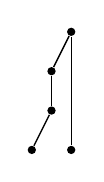
\begin{tikzpicture}[poset,baseline=0pt]
\node[pt] (v0) at (-0.5,0) {};
\node[pt] (v1) at (0.5,0) {};
\node[pt] (v2) at (0,1) {};
\node[pt] (v3) at (0,2) {};
\node[pt] (v4) at (0.5,3) {};
\draw[cov] (v0) -- (v2);
\draw[cov] (v1) -- (v4);
\draw[cov] (v2) -- (v3);
\draw[cov] (v3) -- (v4);
\end{tikzpicture}
\posetsep
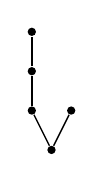
\begin{tikzpicture}[poset,baseline=0pt]
\node[pt] (v0) at (0,0) {};
\node[pt] (v1) at (-0.5,1) {};
\node[pt] (v2) at (0.5,1) {};
\node[pt] (v3) at (-0.5,2) {};
\node[pt] (v4) at (-0.5,3) {};
\draw[cov] (v0) -- (v1);
\draw[cov] (v0) -- (v2);
\draw[cov] (v1) -- (v3);
\draw[cov] (v3) -- (v4);
\end{tikzpicture}
\posetsep

\begin{tikzpicture}[poset,baseline=0pt]
\node[pt] (v0) at (0,0) {};
\node[pt] (v1) at (0,1) {};
\node[pt] (v2) at (0,2) {};
\node[pt] (v3) at (0,3) {};
\node[pt] (v4) at (0,4) {};
\draw[cov] (v0) -- (v1);
\draw[cov] (v1) -- (v2);
\draw[cov] (v2) -- (v3);
\draw[cov] (v3) -- (v4);
\end{tikzpicture}
\end{posetrow}

\classhead{5.2}{19}{t^{5} + t^{4} + t + 1}{$\mathbb{D}_{5}$}{$T_3$, Example~\ref{ex:tamari}}
\begin{posetrow}
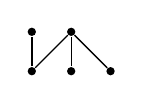
\begin{tikzpicture}[poset,baseline=0pt]
\node[pt] (v0) at (-1,0) {};
\node[pt] (v1) at (0,0) {};
\node[pt] (v2) at (1,0) {};
\node[pt] (v3) at (-1,1) {};
\node[pt] (v4) at (0,1) {};
\draw[cov] (v0) -- (v3);
\draw[cov] (v0) -- (v4);
\draw[cov] (v1) -- (v4);
\draw[cov] (v2) -- (v4);
\end{tikzpicture}
\posetsep
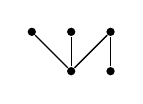
\begin{tikzpicture}[poset,baseline=0pt]
\node[pt] (v0) at (-0.5,0) {};
\node[pt] (v1) at (0.5,0) {};
\node[pt] (v2) at (-1.5,1) {};
\node[pt] (v3) at (-0.5,1) {};
\node[pt] (v4) at (0.5,1) {};
\draw[cov] (v0) -- (v2);
\draw[cov] (v0) -- (v3);
\draw[cov] (v0) -- (v4);
\draw[cov] (v1) -- (v4);
\end{tikzpicture}
\posetsep
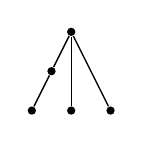
\begin{tikzpicture}[poset,baseline=0pt]
\node[pt] (v0) at (-1,0) {};
\node[pt] (v1) at (0,0) {};
\node[pt] (v2) at (1,0) {};
\node[pt] (v3) at (-0.5,1) {};
\node[pt] (v4) at (0,2) {};
\draw[cov] (v0) -- (v3);
\draw[cov] (v1) -- (v4);
\draw[cov] (v2) -- (v4);
\draw[cov] (v3) -- (v4);
\end{tikzpicture}
\posetsep
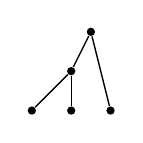
\begin{tikzpicture}[poset,baseline=0pt]
\node[pt] (v0) at (-1,0) {};
\node[pt] (v1) at (0,0) {};
\node[pt] (v2) at (1,0) {};
\node[pt] (v3) at (0,1) {};
\node[pt] (v4) at (0.5,2) {};
\draw[cov] (v0) -- (v3);
\draw[cov] (v1) -- (v3);
\draw[cov] (v2) -- (v4);
\draw[cov] (v3) -- (v4);
\end{tikzpicture}
\posetsep
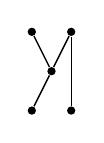
\begin{tikzpicture}[poset,baseline=0pt]
\node[pt] (v0) at (-0.5,0) {};
\node[pt] (v1) at (0.5,0) {};
\node[pt] (v2) at (0,1) {};
\node[pt] (v3) at (-0.5,2) {};
\node[pt] (v4) at (0.5,2) {};
\draw[cov] (v0) -- (v2);
\draw[cov] (v1) -- (v4);
\draw[cov] (v2) -- (v3);
\draw[cov] (v2) -- (v4);
\end{tikzpicture}
\posetsep
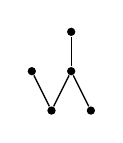
\begin{tikzpicture}[poset,baseline=0pt]
\node[pt] (v0) at (-0.5,0) {};
\node[pt] (v1) at (0.5,0) {};
\node[pt] (v2) at (-1,1) {};
\node[pt] (v3) at (0,1) {};
\node[pt] (v4) at (0,2) {};
\draw[cov] (v0) -- (v2);
\draw[cov] (v0) -- (v3);
\draw[cov] (v1) -- (v3);
\draw[cov] (v3) -- (v4);
\end{tikzpicture}
\posetsep
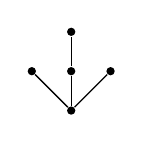
\begin{tikzpicture}[poset,baseline=0pt]
\node[pt] (v0) at (0,0) {};
\node[pt] (v1) at (0,1) {};
\node[pt] (v2) at (-1,1) {};
\node[pt] (v3) at (1,1) {};
\node[pt] (v4) at (0,2) {};
\draw[cov] (v0) -- (v1);
\draw[cov] (v0) -- (v2);
\draw[cov] (v0) -- (v3);
\draw[cov] (v1) -- (v4);
\end{tikzpicture}
\posetsep
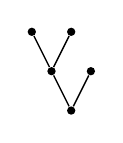
\begin{tikzpicture}[poset,baseline=0pt]
\node[pt] (v0) at (0,0) {};
\node[pt] (v1) at (-0.5,1) {};
\node[pt] (v2) at (0.5,1) {};
\node[pt] (v3) at (-1,2) {};
\node[pt] (v4) at (0,2) {};
\draw[cov] (v0) -- (v1);
\draw[cov] (v0) -- (v2);
\draw[cov] (v1) -- (v3);
\draw[cov] (v1) -- (v4);
\end{tikzpicture}
\posetsep
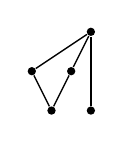
\begin{tikzpicture}[poset,baseline=0pt]
\node[pt] (v0) at (-0.5,0) {};
\node[pt] (v1) at (0.5,0) {};
\node[pt] (v2) at (-1,1) {};
\node[pt] (v3) at (0,1) {};
\node[pt] (v4) at (0.5,2) {};
\draw[cov] (v0) -- (v2);
\draw[cov] (v0) -- (v3);
\draw[cov] (v1) -- (v4);
\draw[cov] (v2) -- (v4);
\draw[cov] (v3) -- (v4);
\end{tikzpicture}
\posetsep
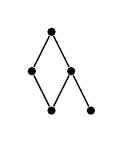
\begin{tikzpicture}[poset,baseline=0pt]
\node[pt] (v0) at (-0.5,0) {};
\node[pt] (v1) at (0.5,0) {};
\node[pt] (v2) at (-1,1) {};
\node[pt] (v3) at (0,1) {};
\node[pt] (v4) at (-0.5,2) {};
\draw[cov] (v0) -- (v2);
\draw[cov] (v0) -- (v3);
\draw[cov] (v1) -- (v3);
\draw[cov] (v2) -- (v4);
\draw[cov] (v3) -- (v4);
\end{tikzpicture}
\posetsep
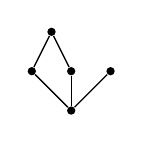
\begin{tikzpicture}[poset,baseline=0pt]
\node[pt] (v0) at (0,0) {};
\node[pt] (v1) at (-1,1) {};
\node[pt] (v2) at (0,1) {};
\node[pt] (v3) at (1,1) {};
\node[pt] (v4) at (-0.5,2) {};
\draw[cov] (v0) -- (v1);
\draw[cov] (v0) -- (v2);
\draw[cov] (v0) -- (v3);
\draw[cov] (v1) -- (v4);
\draw[cov] (v2) -- (v4);
\end{tikzpicture}
\posetsep
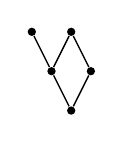
\begin{tikzpicture}[poset,baseline=0pt]
\node[pt] (v0) at (0,0) {};
\node[pt] (v1) at (-0.5,1) {};
\node[pt] (v2) at (0.5,1) {};
\node[pt] (v3) at (-1,2) {};
\node[pt] (v4) at (0,2) {};
\draw[cov] (v0) -- (v1);
\draw[cov] (v0) -- (v2);
\draw[cov] (v1) -- (v3);
\draw[cov] (v1) -- (v4);
\draw[cov] (v2) -- (v4);
\end{tikzpicture}
\posetsep
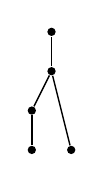
\begin{tikzpicture}[poset,baseline=0pt]
\node[pt] (v0) at (-0.5,0) {};
\node[pt] (v1) at (0.5,0) {};
\node[pt] (v2) at (-0.5,1) {};
\node[pt] (v3) at (0,2) {};
\node[pt] (v4) at (0,3) {};
\draw[cov] (v0) -- (v2);
\draw[cov] (v1) -- (v3);
\draw[cov] (v2) -- (v3);
\draw[cov] (v3) -- (v4);
\end{tikzpicture}
\posetsep
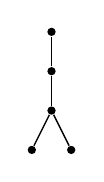
\begin{tikzpicture}[poset,baseline=0pt]
\node[pt] (v0) at (-0.5,0) {};
\node[pt] (v1) at (0.5,0) {};
\node[pt] (v2) at (0,1) {};
\node[pt] (v3) at (0,2) {};
\node[pt] (v4) at (0,3) {};
\draw[cov] (v0) -- (v2);
\draw[cov] (v1) -- (v2);
\draw[cov] (v2) -- (v3);
\draw[cov] (v3) -- (v4);
\end{tikzpicture}
\posetsep
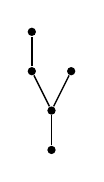
\begin{tikzpicture}[poset,baseline=0pt]
\node[pt] (v0) at (0,0) {};
\node[pt] (v1) at (0,1) {};
\node[pt] (v2) at (-0.5,2) {};
\node[pt] (v3) at (0.5,2) {};
\node[pt] (v4) at (-0.5,3) {};
\draw[cov] (v0) -- (v1);
\draw[cov] (v1) -- (v2);
\draw[cov] (v1) -- (v3);
\draw[cov] (v2) -- (v4);
\end{tikzpicture}
\posetsep
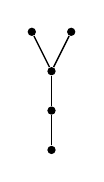
\begin{tikzpicture}[poset,baseline=0pt]
\node[pt] (v0) at (0,0) {};
\node[pt] (v1) at (0,1) {};
\node[pt] (v2) at (0,2) {};
\node[pt] (v3) at (-0.5,3) {};
\node[pt] (v4) at (0.5,3) {};
\draw[cov] (v0) -- (v1);
\draw[cov] (v1) -- (v2);
\draw[cov] (v2) -- (v3);
\draw[cov] (v2) -- (v4);
\end{tikzpicture}
\posetsep
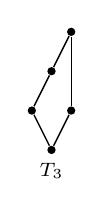
\begin{tikzpicture}[poset,baseline=0pt]
\node[pt] (v0) at (0,0) {};
\node[pt] (v1) at (-0.5,1) {};
\node[pt] (v2) at (0.5,1) {};
\node[pt] (v3) at (0,2) {};
\node[pt] (v4) at (0.5,3) {};
\draw[cov] (v0) -- (v1);
\draw[cov] (v0) -- (v2);
\draw[cov] (v1) -- (v3);
\draw[cov] (v2) -- (v4);
\draw[cov] (v3) -- (v4);
\node[tag] at (current bounding box.south) {$T_3$};
\end{tikzpicture}
\posetsep
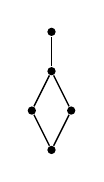
\begin{tikzpicture}[poset,baseline=0pt]
\node[pt] (v0) at (0,0) {};
\node[pt] (v1) at (-0.5,1) {};
\node[pt] (v2) at (0.5,1) {};
\node[pt] (v3) at (0,2) {};
\node[pt] (v4) at (0,3) {};
\draw[cov] (v0) -- (v1);
\draw[cov] (v0) -- (v2);
\draw[cov] (v1) -- (v3);
\draw[cov] (v2) -- (v3);
\draw[cov] (v3) -- (v4);
\end{tikzpicture}
\posetsep
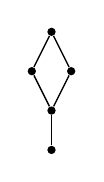
\begin{tikzpicture}[poset,baseline=0pt]
\node[pt] (v0) at (0,0) {};
\node[pt] (v1) at (0,1) {};
\node[pt] (v2) at (-0.5,2) {};
\node[pt] (v3) at (0.5,2) {};
\node[pt] (v4) at (0,3) {};
\draw[cov] (v0) -- (v1);
\draw[cov] (v1) -- (v2);
\draw[cov] (v1) -- (v3);
\draw[cov] (v2) -- (v4);
\draw[cov] (v3) -- (v4);
\end{tikzpicture}
\end{posetrow}

\classhead{5.3}{8}{t^{5} + t^{4} - 2t^{3} - 2t^{2} + t + 1}{$\widetilde{\mathbb{D}}_4$}{}
\begin{posetrow}
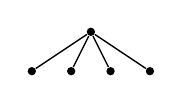
\begin{tikzpicture}[poset,baseline=0pt]
\node[pt] (v0) at (-1.5,0) {};
\node[pt] (v1) at (-0.5,0) {};
\node[pt] (v2) at (0.5,0) {};
\node[pt] (v3) at (1.5,0) {};
\node[pt] (v4) at (0,1) {};
\draw[cov] (v0) -- (v4);
\draw[cov] (v1) -- (v4);
\draw[cov] (v2) -- (v4);
\draw[cov] (v3) -- (v4);
\end{tikzpicture}
\posetsep
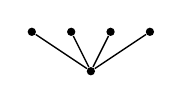
\begin{tikzpicture}[poset,baseline=0pt]
\node[pt] (v0) at (0,0) {};
\node[pt] (v1) at (-1.5,1) {};
\node[pt] (v2) at (-0.5,1) {};
\node[pt] (v3) at (0.5,1) {};
\node[pt] (v4) at (1.5,1) {};
\draw[cov] (v0) -- (v1);
\draw[cov] (v0) -- (v2);
\draw[cov] (v0) -- (v3);
\draw[cov] (v0) -- (v4);
\end{tikzpicture}
\posetsep
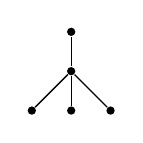
\begin{tikzpicture}[poset,baseline=0pt]
\node[pt] (v0) at (-1,0) {};
\node[pt] (v1) at (0,0) {};
\node[pt] (v2) at (1,0) {};
\node[pt] (v3) at (0,1) {};
\node[pt] (v4) at (0,2) {};
\draw[cov] (v0) -- (v3);
\draw[cov] (v1) -- (v3);
\draw[cov] (v2) -- (v3);
\draw[cov] (v3) -- (v4);
\end{tikzpicture}
\posetsep
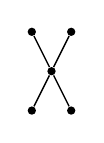
\begin{tikzpicture}[poset,baseline=0pt]
\node[pt] (v0) at (-0.5,0) {};
\node[pt] (v1) at (0.5,0) {};
\node[pt] (v2) at (0,1) {};
\node[pt] (v3) at (-0.5,2) {};
\node[pt] (v4) at (0.5,2) {};
\draw[cov] (v0) -- (v2);
\draw[cov] (v1) -- (v2);
\draw[cov] (v2) -- (v3);
\draw[cov] (v2) -- (v4);
\end{tikzpicture}
\posetsep
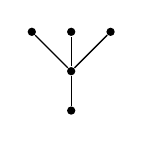
\begin{tikzpicture}[poset,baseline=0pt]
\node[pt] (v0) at (0,0) {};
\node[pt] (v1) at (0,1) {};
\node[pt] (v2) at (-1,2) {};
\node[pt] (v3) at (0,2) {};
\node[pt] (v4) at (1,2) {};
\draw[cov] (v0) -- (v1);
\draw[cov] (v1) -- (v2);
\draw[cov] (v1) -- (v3);
\draw[cov] (v1) -- (v4);
\end{tikzpicture}
\posetsep
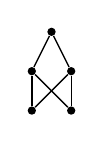
\begin{tikzpicture}[poset,baseline=0pt]
\node[pt] (v0) at (-0.5,0) {};
\node[pt] (v1) at (0.5,0) {};
\node[pt] (v2) at (-0.5,1) {};
\node[pt] (v3) at (0.5,1) {};
\node[pt] (v4) at (0,2) {};
\draw[cov] (v0) -- (v2);
\draw[cov] (v0) -- (v3);
\draw[cov] (v1) -- (v2);
\draw[cov] (v1) -- (v3);
\draw[cov] (v2) -- (v4);
\draw[cov] (v3) -- (v4);
\end{tikzpicture}
\posetsep
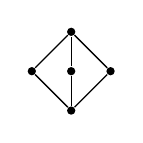
\begin{tikzpicture}[poset,baseline=0pt]
\node[pt] (v0) at (0,0) {};
\node[pt] (v1) at (-1,1) {};
\node[pt] (v2) at (0,1) {};
\node[pt] (v3) at (1,1) {};
\node[pt] (v4) at (0,2) {};
\draw[cov] (v0) -- (v1);
\draw[cov] (v0) -- (v2);
\draw[cov] (v0) -- (v3);
\draw[cov] (v1) -- (v4);
\draw[cov] (v2) -- (v4);
\draw[cov] (v3) -- (v4);
\end{tikzpicture}
\posetsep
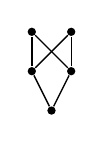
\begin{tikzpicture}[poset,baseline=0pt]
\node[pt] (v0) at (0,0) {};
\node[pt] (v1) at (-0.5,1) {};
\node[pt] (v2) at (0.5,1) {};
\node[pt] (v3) at (-0.5,2) {};
\node[pt] (v4) at (0.5,2) {};
\draw[cov] (v0) -- (v1);
\draw[cov] (v0) -- (v2);
\draw[cov] (v1) -- (v3);
\draw[cov] (v1) -- (v4);
\draw[cov] (v2) -- (v3);
\draw[cov] (v2) -- (v4);
\end{tikzpicture}
\end{posetrow}

\classhead{5.4}{1}{t^{5} - t^{3} - t^{2} + 1}{$\widetilde{\mathbb{A}}_{2,3}$}{}
\begin{posetrow}
\begin{tikzpicture}[poset,baseline=0pt]
\node[pt] (v0) at (-0.5,0) {};
\node[pt] (v1) at (0.5,0) {};
\node[pt] (v2) at (-1,1) {};
\node[pt] (v3) at (0,1) {};
\node[pt] (v4) at (0.5,2) {};
\draw[cov] (v0) -- (v2);
\draw[cov] (v0) -- (v3);
\draw[cov] (v1) -- (v3);
\draw[cov] (v1) -- (v4);
\draw[cov] (v2) -- (v4);
\end{tikzpicture}
\end{posetrow}

\classhead{5.5}{4}{t^{5} - 3t^{3} - 3t^{2} + 1}{}{}
\begin{posetrow}
\begin{tikzpicture}[poset,baseline=0pt]
\node[pt] (v0) at (-1,0) {};
\node[pt] (v1) at (0,0) {};
\node[pt] (v2) at (1,0) {};
\node[pt] (v3) at (-1,1) {};
\node[pt] (v4) at (0,1) {};
\draw[cov] (v0) -- (v3);
\draw[cov] (v0) -- (v4);
\draw[cov] (v1) -- (v3);
\draw[cov] (v1) -- (v4);
\draw[cov] (v2) -- (v4);
\end{tikzpicture}
\posetsep
\begin{tikzpicture}[poset,baseline=0pt]
\node[pt] (v0) at (-0.5,0) {};
\node[pt] (v1) at (0.5,0) {};
\node[pt] (v2) at (-1.5,1) {};
\node[pt] (v3) at (-0.5,1) {};
\node[pt] (v4) at (0.5,1) {};
\draw[cov] (v0) -- (v2);
\draw[cov] (v0) -- (v3);
\draw[cov] (v0) -- (v4);
\draw[cov] (v1) -- (v3);
\draw[cov] (v1) -- (v4);
\end{tikzpicture}
\posetsep
\begin{tikzpicture}[poset,baseline=0pt]
\node[pt] (v0) at (-0.5,0) {};
\node[pt] (v1) at (0.5,0) {};
\node[pt] (v2) at (-0.5,1) {};
\node[pt] (v3) at (-0.5,2) {};
\node[pt] (v4) at (0.5,2) {};
\draw[cov] (v0) -- (v2);
\draw[cov] (v1) -- (v3);
\draw[cov] (v1) -- (v4);
\draw[cov] (v2) -- (v3);
\draw[cov] (v2) -- (v4);
\end{tikzpicture}
\posetsep
\begin{tikzpicture}[poset,baseline=0pt]
\node[pt] (v0) at (-0.5,0) {};
\node[pt] (v1) at (0.5,0) {};
\node[pt] (v2) at (-0.5,1) {};
\node[pt] (v3) at (0.5,1) {};
\node[pt] (v4) at (-0.5,2) {};
\draw[cov] (v0) -- (v2);
\draw[cov] (v0) -- (v3);
\draw[cov] (v1) -- (v2);
\draw[cov] (v1) -- (v3);
\draw[cov] (v2) -- (v4);
\end{tikzpicture}
\end{posetrow}

\classhead{5.6}{2}{t^{5} - t^{4} - 8t^{3} - 8t^{2} - t + 1}{}{$2\oplus3$, $3\oplus2$, Proposition~\ref{prop:ordinal-sums}}
\begin{posetrow}
\begin{tikzpicture}[poset,baseline=0pt]
\node[pt] (v0) at (-1,0) {};
\node[pt] (v1) at (0,0) {};
\node[pt] (v2) at (1,0) {};
\node[pt] (v3) at (-0.5,1) {};
\node[pt] (v4) at (0.5,1) {};
\draw[cov] (v0) -- (v3);
\draw[cov] (v0) -- (v4);
\draw[cov] (v1) -- (v3);
\draw[cov] (v1) -- (v4);
\draw[cov] (v2) -- (v3);
\draw[cov] (v2) -- (v4);
\node[tag] at (current bounding box.south) {$3\oplus2$};
\end{tikzpicture}
\posetsep
\begin{tikzpicture}[poset,baseline=0pt]
\node[pt] (v0) at (-0.5,0) {};
\node[pt] (v1) at (0.5,0) {};
\node[pt] (v2) at (-1,1) {};
\node[pt] (v3) at (0,1) {};
\node[pt] (v4) at (1,1) {};
\draw[cov] (v0) -- (v2);
\draw[cov] (v0) -- (v3);
\draw[cov] (v0) -- (v4);
\draw[cov] (v1) -- (v2);
\draw[cov] (v1) -- (v3);
\draw[cov] (v1) -- (v4);
\node[tag] at (current bounding box.south) {$2\oplus3$};
\end{tikzpicture}
\end{posetrow}

\subsection{Connected posets with six elements}
\label{app:six}
Table~\ref{tab:app-six} lists the $23$ classes of the $238$ connected posets with six elements, with one representative each; when a class contains the orientations of a tree, the representative is one of them. Two pairs of rows have the same Coxeter polynomial. The classes 6.6 and 6.20 are separated by the Smith normal form of $C_P+C_P^{T}$ (Section~\ref{Derived invariants and the census}), which is $\operatorname{diag}(1,1,1,1,6,0)$ and $\operatorname{diag}(1,1,1,1,4,0)$, respectively. The classes $\alpha$ and $\beta$ of Section~\ref{the case of six elements} are not separated by any of our invariants.

{\setlength{\tabcolsep}{4pt}
\begin{longtable}{c c c >{$}l<{$} c >{\raggedright\arraybackslash}p{2.9cm}}
\caption{The $\sim_L$-classes of connected posets with six elements.}\label{tab:app-six}\\
\toprule class & representative & size & \chi_P(t) & type & remarks \\ \midrule \endfirsthead
\toprule class & representative & size & \chi_P(t) & type & remarks \\ \midrule \endhead
\bottomrule \endfoot
6.1 & \begin{tikzpicture}[poset,baseline={([yshift=-.6ex]current bounding box.center)}]
\node[pt] (v0) at (-1,0) {};
\node[pt] (v1) at (0,0) {};
\node[pt] (v2) at (1,0) {};
\node[pt] (v3) at (-1.5,1) {};
\node[pt] (v4) at (-0.5,1) {};
\node[pt] (v5) at (0.5,1) {};
\draw[cov] (v0) -- (v3);
\draw[cov] (v0) -- (v4);
\draw[cov] (v1) -- (v4);
\draw[cov] (v1) -- (v5);
\draw[cov] (v2) -- (v5);
\path ([yshift=-4pt]current bounding box.south) ([yshift=4pt]current bounding box.north);
\end{tikzpicture} & 16 & t^{6} + t^{5} + t^{4} + t^{3} + t^{2} + t + 1 & $\mathbb{A}_{6}$ &  \\[2pt]
6.2 & \begin{tikzpicture}[poset,baseline={([yshift=-.6ex]current bounding box.center)}]
\node[pt] (v0) at (-0.5,0) {};
\node[pt] (v1) at (-1.5,0) {};
\node[pt] (v2) at (0.5,0) {};
\node[pt] (v3) at (1.5,0) {};
\node[pt] (v4) at (-0.5,1) {};
\node[pt] (v5) at (0.5,1) {};
\draw[cov] (v0) -- (v4);
\draw[cov] (v0) -- (v5);
\draw[cov] (v1) -- (v4);
\draw[cov] (v2) -- (v5);
\draw[cov] (v3) -- (v5);
\path ([yshift=-4pt]current bounding box.south) ([yshift=4pt]current bounding box.north);
\end{tikzpicture} & 43 & t^{6} + t^{5} + t + 1 & $\mathbb{D}_{6}$ &  \\[2pt]
6.3 & \begin{tikzpicture}[poset,baseline={([yshift=-.6ex]current bounding box.center)}]
\node[pt] (v0) at (0,0) {};
\node[pt] (v1) at (-1,0) {};
\node[pt] (v2) at (1,0) {};
\node[pt] (v3) at (0,1) {};
\node[pt] (v4) at (-1,1) {};
\node[pt] (v5) at (1,1) {};
\draw[cov] (v0) -- (v3);
\draw[cov] (v0) -- (v4);
\draw[cov] (v0) -- (v5);
\draw[cov] (v1) -- (v4);
\draw[cov] (v2) -- (v5);
\path ([yshift=-4pt]current bounding box.south) ([yshift=4pt]current bounding box.north);
\end{tikzpicture} & 43 & t^{6} + t^{5} - t^{3} + t + 1 & $\mathbb{E}_6$ &  \\[2pt]
6.4 & \begin{tikzpicture}[poset,baseline={([yshift=-.6ex]current bounding box.center)}]
\node[pt] (v0) at (-1,0) {};
\node[pt] (v1) at (0,0) {};
\node[pt] (v2) at (1,0) {};
\node[pt] (v3) at (-2,1) {};
\node[pt] (v4) at (-1,1) {};
\node[pt] (v5) at (0,1) {};
\draw[cov] (v0) -- (v3);
\draw[cov] (v0) -- (v4);
\draw[cov] (v0) -- (v5);
\draw[cov] (v1) -- (v5);
\draw[cov] (v2) -- (v5);
\path ([yshift=-4pt]current bounding box.south) ([yshift=4pt]current bounding box.north);
\end{tikzpicture} & 29 & t^{6} + t^{5} - t^{4} - 2t^{3} - t^{2} + t + 1 & $\widetilde{\mathbb{D}}_{5}$ &  \\[2pt]
6.5 & \begin{tikzpicture}[poset,baseline={([yshift=-.6ex]current bounding box.center)}]
\node[pt] (v0) at (-1,0) {};
\node[pt] (v1) at (0,0) {};
\node[pt] (v2) at (1,0) {};
\node[pt] (v3) at (-1,1) {};
\node[pt] (v4) at (0,1) {};
\node[pt] (v5) at (1,1) {};
\draw[cov] (v0) -- (v3);
\draw[cov] (v0) -- (v4);
\draw[cov] (v1) -- (v3);
\draw[cov] (v1) -- (v5);
\draw[cov] (v2) -- (v4);
\draw[cov] (v2) -- (v5);
\path ([yshift=-4pt]current bounding box.south) ([yshift=4pt]current bounding box.north);
\end{tikzpicture} & 3 & t^{6} - 2t^{3} + 1 & $\widetilde{\mathbb{A}}_{3,3}$ &  \\[2pt]
6.6 & \begin{tikzpicture}[poset,baseline={([yshift=-.6ex]current bounding box.center)}]
\node[pt] (v0) at (-0.5,0) {};
\node[pt] (v1) at (0.5,0) {};
\node[pt] (v2) at (-0.5,1) {};
\node[pt] (v3) at (0.5,1) {};
\node[pt] (v4) at (-0.5,2) {};
\node[pt] (v5) at (0.5,2) {};
\draw[cov] (v0) -- (v2);
\draw[cov] (v0) -- (v5);
\draw[cov] (v1) -- (v3);
\draw[cov] (v1) -- (v4);
\draw[cov] (v2) -- (v4);
\draw[cov] (v3) -- (v5);
\path ([yshift=-4pt]current bounding box.south) ([yshift=4pt]current bounding box.north);
\end{tikzpicture} & 2 & t^{6} - t^{4} - t^{2} + 1 & $\widetilde{\mathbb{A}}_{2,4}$ &  \\[2pt]
6.7 & \begin{tikzpicture}[poset,baseline={([yshift=-.6ex]current bounding box.center)}]
\node[pt] (v0) at (-1.5,0) {};
\node[pt] (v1) at (-0.5,0) {};
\node[pt] (v2) at (0.5,0) {};
\node[pt] (v3) at (1.5,0) {};
\node[pt] (v4) at (-1,1) {};
\node[pt] (v5) at (0,1) {};
\draw[cov] (v0) -- (v4);
\draw[cov] (v0) -- (v5);
\draw[cov] (v1) -- (v5);
\draw[cov] (v2) -- (v5);
\draw[cov] (v3) -- (v5);
\path ([yshift=-4pt]current bounding box.south) ([yshift=4pt]current bounding box.north);
\end{tikzpicture} & 33 & t^{6} + t^{5} - 2t^{4} - 4t^{3} - 2t^{2} + t + 1 & wild &  \\[2pt]
6.8 & \begin{tikzpicture}[poset,baseline={([yshift=-.6ex]current bounding box.center)}]
\node[pt] (v0) at (-2,0) {};
\node[pt] (v1) at (-1,0) {};
\node[pt] (v2) at (0,0) {};
\node[pt] (v3) at (1,0) {};
\node[pt] (v4) at (2,0) {};
\node[pt] (v5) at (0,1) {};
\draw[cov] (v0) -- (v5);
\draw[cov] (v1) -- (v5);
\draw[cov] (v2) -- (v5);
\draw[cov] (v3) -- (v5);
\draw[cov] (v4) -- (v5);
\path ([yshift=-4pt]current bounding box.south) ([yshift=4pt]current bounding box.north);
\end{tikzpicture} & 11 & t^{6} + t^{5} - 5t^{4} - 10t^{3} - 5t^{2} + t + 1 & wild &  \\[2pt]
6.9 & \begin{tikzpicture}[poset,baseline={([yshift=-.6ex]current bounding box.center)}]
\node[pt] (v0) at (-1.5,0) {};
\node[pt] (v1) at (-0.5,0) {};
\node[pt] (v2) at (0.5,0) {};
\node[pt] (v3) at (1.5,0) {};
\node[pt] (v4) at (-1,1) {};
\node[pt] (v5) at (0,1) {};
\draw[cov] (v0) -- (v4);
\draw[cov] (v0) -- (v5);
\draw[cov] (v1) -- (v4);
\draw[cov] (v1) -- (v5);
\draw[cov] (v2) -- (v5);
\draw[cov] (v3) -- (v5);
\path ([yshift=-4pt]current bounding box.south) ([yshift=4pt]current bounding box.north);
\end{tikzpicture} & 8 & t^{6} - 5t^{4} - 8t^{3} - 5t^{2} + 1 & -- &  \\[2pt]
6.10 & \begin{tikzpicture}[poset,baseline={([yshift=-.6ex]current bounding box.center)}]
\node[pt] (v0) at (0,0) {};
\node[pt] (v1) at (-1,0) {};
\node[pt] (v2) at (1,0) {};
\node[pt] (v3) at (-1,1) {};
\node[pt] (v4) at (0,1) {};
\node[pt] (v5) at (1,1) {};
\draw[cov] (v0) -- (v3);
\draw[cov] (v0) -- (v4);
\draw[cov] (v0) -- (v5);
\draw[cov] (v1) -- (v3);
\draw[cov] (v1) -- (v4);
\draw[cov] (v2) -- (v5);
\path ([yshift=-4pt]current bounding box.south) ([yshift=4pt]current bounding box.north);
\end{tikzpicture} & 8 & t^{6} - 3t^{4} - 4t^{3} - 3t^{2} + 1 & -- &  \\[2pt]
6.11 & \begin{tikzpicture}[poset,baseline={([yshift=-.6ex]current bounding box.center)}]
\node[pt] (v0) at (-0.5,0) {};
\node[pt] (v1) at (0.5,0) {};
\node[pt] (v2) at (-1.5,0) {};
\node[pt] (v3) at (1.5,0) {};
\node[pt] (v4) at (-0.5,1) {};
\node[pt] (v5) at (0.5,1) {};
\draw[cov] (v0) -- (v4);
\draw[cov] (v0) -- (v5);
\draw[cov] (v1) -- (v4);
\draw[cov] (v1) -- (v5);
\draw[cov] (v2) -- (v4);
\draw[cov] (v3) -- (v5);
\path ([yshift=-4pt]current bounding box.south) ([yshift=4pt]current bounding box.north);
\end{tikzpicture} & 6 & t^{6} - 4t^{4} - 6t^{3} - 4t^{2} + 1 & -- &  \\[2pt]
6.12 & \begin{tikzpicture}[poset,baseline={([yshift=-.6ex]current bounding box.center)}]
\node[pt] (v0) at (-1.5,0) {};
\node[pt] (v1) at (-0.5,0) {};
\node[pt] (v2) at (0.5,0) {};
\node[pt] (v3) at (1.5,0) {};
\node[pt] (v4) at (-1,1) {};
\node[pt] (v5) at (0,1) {};
\draw[cov] (v0) -- (v4);
\draw[cov] (v0) -- (v5);
\draw[cov] (v1) -- (v4);
\draw[cov] (v1) -- (v5);
\draw[cov] (v2) -- (v4);
\draw[cov] (v2) -- (v5);
\draw[cov] (v3) -- (v5);
\path ([yshift=-4pt]current bounding box.south) ([yshift=4pt]current bounding box.north);
\end{tikzpicture} & 4 & t^{6} - t^{5} - 10t^{4} - 16t^{3} - 10t^{2} - t + 1 & -- &  \\[2pt]
6.13 & \begin{tikzpicture}[poset,baseline={([yshift=-.6ex]current bounding box.center)}]
\node[pt] (v0) at (-1,0) {};
\node[pt] (v1) at (0,0) {};
\node[pt] (v2) at (1,0) {};
\node[pt] (v3) at (-1.5,1) {};
\node[pt] (v4) at (-0.5,1) {};
\node[pt] (v5) at (0.5,1) {};
\draw[cov] (v0) -- (v3);
\draw[cov] (v0) -- (v4);
\draw[cov] (v0) -- (v5);
\draw[cov] (v1) -- (v3);
\draw[cov] (v1) -- (v4);
\draw[cov] (v1) -- (v5);
\draw[cov] (v2) -- (v5);
\path ([yshift=-4pt]current bounding box.south) ([yshift=4pt]current bounding box.north);
\end{tikzpicture} & 4 & t^{6} - t^{5} - 9t^{4} - 14t^{3} - 9t^{2} - t + 1 & -- &  \\[2pt]
6.14 & \begin{tikzpicture}[poset,baseline={([yshift=-.6ex]current bounding box.center)}]
\node[pt] (v0) at (-1,0) {};
\node[pt] (v1) at (0,0) {};
\node[pt] (v2) at (1,0) {};
\node[pt] (v3) at (-1.5,1) {};
\node[pt] (v4) at (-0.5,1) {};
\node[pt] (v5) at (0,2) {};
\draw[cov] (v0) -- (v3);
\draw[cov] (v0) -- (v4);
\draw[cov] (v1) -- (v4);
\draw[cov] (v1) -- (v5);
\draw[cov] (v2) -- (v4);
\draw[cov] (v2) -- (v5);
\draw[cov] (v3) -- (v5);
\path ([yshift=-4pt]current bounding box.south) ([yshift=4pt]current bounding box.north);
\end{tikzpicture} & 4 & t^{6} - t^{5} - 6t^{4} - 8t^{3} - 6t^{2} - t + 1 & -- &  \\[2pt]
6.15 & \begin{tikzpicture}[poset,baseline={([yshift=-.6ex]current bounding box.center)}]
\node[pt] (v0) at (-1,0) {};
\node[pt] (v1) at (0,0) {};
\node[pt] (v2) at (1,0) {};
\node[pt] (v3) at (-1.5,1) {};
\node[pt] (v4) at (-0.5,1) {};
\node[pt] (v5) at (0.5,1) {};
\draw[cov] (v0) -- (v3);
\draw[cov] (v0) -- (v4);
\draw[cov] (v0) -- (v5);
\draw[cov] (v1) -- (v4);
\draw[cov] (v1) -- (v5);
\draw[cov] (v2) -- (v5);
\path ([yshift=-4pt]current bounding box.south) ([yshift=4pt]current bounding box.north);
\end{tikzpicture} & 4 & t^{6} - 4t^{4} - 7t^{3} - 4t^{2} + 1 & -- &  \\[2pt]
6.16 & \begin{tikzpicture}[poset,baseline={([yshift=-.6ex]current bounding box.center)}]
\node[pt] (v0) at (-1.5,0) {};
\node[pt] (v1) at (-0.5,0) {};
\node[pt] (v2) at (0.5,0) {};
\node[pt] (v3) at (1.5,0) {};
\node[pt] (v4) at (-0.5,1) {};
\node[pt] (v5) at (0.5,1) {};
\draw[cov] (v0) -- (v4);
\draw[cov] (v0) -- (v5);
\draw[cov] (v1) -- (v4);
\draw[cov] (v1) -- (v5);
\draw[cov] (v2) -- (v4);
\draw[cov] (v2) -- (v5);
\draw[cov] (v3) -- (v4);
\draw[cov] (v3) -- (v5);
\path ([yshift=-4pt]current bounding box.south) ([yshift=4pt]current bounding box.north);
\end{tikzpicture} & 2 & t^{6} - 2t^{5} - 17t^{4} - 28t^{3} - 17t^{2} - 2t + 1 & -- & $2\oplus4$, $4\oplus2$, Proposition~\ref{prop:ordinal-sums} \\[2pt]
6.17 & \begin{tikzpicture}[poset,baseline={([yshift=-.6ex]current bounding box.center)}]
\node[pt] (v0) at (-1,0) {};
\node[pt] (v1) at (0,0) {};
\node[pt] (v2) at (1,0) {};
\node[pt] (v3) at (-1,1) {};
\node[pt] (v4) at (0,1) {};
\node[pt] (v5) at (1,1) {};
\draw[cov] (v0) -- (v3);
\draw[cov] (v0) -- (v4);
\draw[cov] (v0) -- (v5);
\draw[cov] (v1) -- (v3);
\draw[cov] (v1) -- (v4);
\draw[cov] (v1) -- (v5);
\draw[cov] (v2) -- (v3);
\draw[cov] (v2) -- (v4);
\draw[cov] (v2) -- (v5);
\path ([yshift=-4pt]current bounding box.south) ([yshift=4pt]current bounding box.north);
\end{tikzpicture} & 1 & t^{6} - 3t^{5} - 21t^{4} - 34t^{3} - 21t^{2} - 3t + 1 & -- & $3\oplus3$, Proposition~\ref{prop:ordinal-sums} \\[2pt]
6.18 & \begin{tikzpicture}[poset,baseline={([yshift=-.6ex]current bounding box.center)}]
\node[pt] (v0) at (-1,0) {};
\node[pt] (v1) at (0,0) {};
\node[pt] (v2) at (1,0) {};
\node[pt] (v3) at (-1,1) {};
\node[pt] (v4) at (0,1) {};
\node[pt] (v5) at (1,1) {};
\draw[cov] (v0) -- (v3);
\draw[cov] (v0) -- (v4);
\draw[cov] (v0) -- (v5);
\draw[cov] (v1) -- (v3);
\draw[cov] (v1) -- (v4);
\draw[cov] (v1) -- (v5);
\draw[cov] (v2) -- (v4);
\draw[cov] (v2) -- (v5);
\path ([yshift=-4pt]current bounding box.south) ([yshift=4pt]current bounding box.north);
\end{tikzpicture} & 1 & t^{6} - 2t^{5} - 13t^{4} - 20t^{3} - 13t^{2} - 2t + 1 & -- &  \\[2pt]
6.19 & \begin{tikzpicture}[poset,baseline={([yshift=-.6ex]current bounding box.center)}]
\node[pt] (v0) at (0,0) {};
\node[pt] (v1) at (-1,0) {};
\node[pt] (v2) at (1,0) {};
\node[pt] (v3) at (-1,1) {};
\node[pt] (v4) at (1,1) {};
\node[pt] (v5) at (0,1) {};
\draw[cov] (v0) -- (v3);
\draw[cov] (v0) -- (v4);
\draw[cov] (v0) -- (v5);
\draw[cov] (v1) -- (v3);
\draw[cov] (v1) -- (v5);
\draw[cov] (v2) -- (v4);
\draw[cov] (v2) -- (v5);
\path ([yshift=-4pt]current bounding box.south) ([yshift=4pt]current bounding box.north);
\end{tikzpicture} & 1 & t^{6} - t^{5} - 6t^{4} - 9t^{3} - 6t^{2} - t + 1 & -- &  \\[2pt]
6.20 & \begin{tikzpicture}[poset,baseline={([yshift=-.6ex]current bounding box.center)}]
\node[pt] (v0) at (-0.5,0) {};
\node[pt] (v1) at (0.5,0) {};
\node[pt] (v2) at (-2,1) {};
\node[pt] (v3) at (-1,1) {};
\node[pt] (v4) at (0,1) {};
\node[pt] (v5) at (0.5,2) {};
\draw[cov] (v0) -- (v2);
\draw[cov] (v0) -- (v3);
\draw[cov] (v0) -- (v4);
\draw[cov] (v1) -- (v4);
\draw[cov] (v1) -- (v5);
\draw[cov] (v2) -- (v5);
\draw[cov] (v3) -- (v5);
\path ([yshift=-4pt]current bounding box.south) ([yshift=4pt]current bounding box.north);
\end{tikzpicture} & 1 & t^{6} - t^{4} - t^{2} + 1 & -- &  \\[2pt]
6.21 & \begin{tikzpicture}[poset,baseline={([yshift=-.6ex]current bounding box.center)}]
\node[pt] (v0) at (-0.5,0) {};
\node[pt] (v1) at (0.5,0) {};
\node[pt] (v2) at (-0.5,1) {};
\node[pt] (v3) at (0.5,1) {};
\node[pt] (v4) at (-0.5,2) {};
\node[pt] (v5) at (0.5,2) {};
\draw[cov] (v0) -- (v2);
\draw[cov] (v0) -- (v3);
\draw[cov] (v1) -- (v2);
\draw[cov] (v1) -- (v3);
\draw[cov] (v2) -- (v4);
\draw[cov] (v2) -- (v5);
\draw[cov] (v3) -- (v4);
\draw[cov] (v3) -- (v5);
\path ([yshift=-4pt]current bounding box.south) ([yshift=4pt]current bounding box.north);
\end{tikzpicture} & 1 & t^{6} + 2t^{5} - t^{4} - 4t^{3} - t^{2} + 2t + 1 & -- & $2\oplus2\oplus2$, Proposition~\ref{prop:ordinal-sums} \\[2pt]
$\alpha$ & \begin{tikzpicture}[poset,baseline={([yshift=-.6ex]current bounding box.center)}]
\node[pt] (v0) at (-0.5,0) {};
\node[pt] (v1) at (0.5,0) {};
\node[pt] (v2) at (-1,1) {};
\node[pt] (v3) at (0,1) {};
\node[pt] (v4) at (-0.5,2) {};
\node[pt] (v5) at (0.5,2) {};
\draw[cov] (v0) -- (v2);
\draw[cov] (v0) -- (v3);
\draw[cov] (v1) -- (v3);
\draw[cov] (v1) -- (v5);
\draw[cov] (v2) -- (v4);
\draw[cov] (v2) -- (v5);
\draw[cov] (v3) -- (v4);
\path ([yshift=-4pt]current bounding box.south) ([yshift=4pt]current bounding box.north);
\end{tikzpicture} & 3 & t^{6} - 2t^{4} - 3t^{3} - 2t^{2} + 1 & -- & $P_\alpha$ of Section~\ref{the case of six elements} \\[2pt]
$\beta$ & \begin{tikzpicture}[poset,baseline={([yshift=-.6ex]current bounding box.center)}]
\node[pt] (v0) at (0,0) {};
\node[pt] (v1) at (-1,0) {};
\node[pt] (v2) at (1,0) {};
\node[pt] (v3) at (0.5,1) {};
\node[pt] (v4) at (1.5,1) {};
\node[pt] (v5) at (0,2) {};
\draw[cov] (v0) -- (v3);
\draw[cov] (v0) -- (v5);
\draw[cov] (v1) -- (v5);
\draw[cov] (v2) -- (v3);
\draw[cov] (v2) -- (v4);
\draw[cov] (v4) -- (v5);
\path ([yshift=-4pt]current bounding box.south) ([yshift=4pt]current bounding box.north);
\end{tikzpicture} & 10 & t^{6} - 2t^{4} - 3t^{3} - 2t^{2} + 1 & -- & $P_\beta$ of Section~\ref{the case of six elements} \\[2pt]
\end{longtable}}

\subsection{Connected posets with seven to nine elements}
\label{app:large}
For $n = 7, 8, 9$ there are $117$, $1\,284$ and $21\,197$ classes
(Table~\ref{tab:small-poset-census}), too many to be listed here. They are available in the
repository \url{https://github.com/chiara-ascenzi/UDE-posets} in machine-readable form: for each $n$, a file with one line per
connected poset, containing the digraph6 string of its Hasse diagram and the label of its
$\sim_L$-class. The digraph6 format, used by nauty~\cite{McKayPiperno}, encodes a directed graph as a
single line of printable ASCII characters.

